\documentclass[12pt,a4paper]{article}

% -------------------------------------------------------
% PACKAGES
% -------------------------------------------------------
\usepackage{amsmath}
\usepackage{amssymb}
\usepackage{geometry}
\geometry{margin=2.5cm}
\usepackage{booktabs}
\usepackage{xcolor}
\usepackage{hyperref}
\usepackage{listings}
\usepackage{pgfplots}
\pgfplotsset{compat=1.18}
\usepackage{tcolorbox}
\tcbuselibrary{skins, breakable}
\usepackage{enumitem}
\usepackage{fancyhdr}
\usepackage{tikz}
\usepackage{array}
\usepackage{subcaption}

% -------------------------------------------------------
% TCOLORBOX ENVIRONMENTS
% -------------------------------------------------------
\newtcolorbox{curiositybox}[1]{colback=yellow!10, colframe=orange!80!black, fonttitle=\bfseries, title=#1, breakable}
\newtcolorbox{infobox}[1]{colback=blue!5, colframe=blue!60!black, fonttitle=\bfseries, title=#1, breakable}
\newtcolorbox{mistakebox}[1]{colback=red!5, colframe=red!60!black, fonttitle=\bfseries, title=#1, breakable}
\newtcolorbox{learnbox}[1]{colback=green!5, colframe=green!60!black, fonttitle=\bfseries, title=#1, breakable}

% -------------------------------------------------------
% LISTINGS (Python)
% -------------------------------------------------------
\lstset{language=Python, basicstyle=\ttfamily\small, keywordstyle=\color{blue},
        commentstyle=\color{gray}, stringstyle=\color{orange},
        showstringspaces=false, numbers=left, numberstyle=\tiny,
        breaklines=true, frame=single}

% -------------------------------------------------------
% FANCYHDR
% -------------------------------------------------------
\pagestyle{fancy}
\fancyhf{}
\lhead{Topic 02: Dirichlet Conditions}
\rhead{Unit V --- Fourier Series \& Transforms}
\cfoot{\thepage}

% -------------------------------------------------------
% TITLE
% -------------------------------------------------------
\title{Topic 02: Dirichlet Conditions for Existence of Fourier Series \\
       \large Unit V --- Fourier Series \& Fourier Transforms}
\author{23A54201 --- Mathematics IV (Transform Techniques) \\
        JNTUA College of Engineering (Autonomous)}
\date{}

% -------------------------------------------------------
% DOCUMENT
% -------------------------------------------------------
\begin{document}

\maketitle
\tableofcontents
\newpage

% ============================================================
% SECTION 1: OPENING HOOK
% ============================================================
\section{Opening Hook}

\begin{curiositybox}{Hook}
In Topic 01 we assumed the Fourier series converges to $f(x)$ and went ahead. But a student asks: what if the function has infinitely many jumps? Or a wild infinite spike? Can we still trust the Fourier series to converge? Dirichlet answered this question in 1829 by writing down three simple conditions --- if a function satisfies them, its Fourier series is GUARANTEED to converge. And nearly every function you will ever meet in engineering passes these conditions easily.
\end{curiositybox}

% ============================================================
% SECTION 2: WHY THIS TOPIC EXISTS
% ============================================================
\section{Why This Topic Exists}

``Before we begin, here is the honest answer to why you are reading this\ldots''

When you compute Euler coefficients $a_0$, $a_n$, $b_n$ and write down the Fourier series
\[
   \frac{a_0}{2} + \sum_{n=1}^{\infty}\bigl(a_n \cos nx + b_n \sin nx\bigr),
\]
you are producing a formal series. The question ``does this series actually equal $f(x)$?'' is a completely separate question --- and one that cannot be ignored in engineering.
Dirichlet conditions are the practical three-item checklist you run \emph{before} trusting the series in a model, a circuit analysis, or a signal-processing algorithm.

\medskip
\begin{center}
\begin{tabular}{@{}p{7cm}p{7cm}@{}}
\toprule
\textbf{Mistake} & \textbf{Consequence} \\
\midrule
Applying Fourier series without checking validity
  & Potentially using a divergent or incorrect series in an engineering model \\
\midrule
Confusing Dirichlet conditions with the existence theorem for Laplace transforms
  & Mixing up two completely separate sets of conditions \\
\midrule
Forgetting convergence at discontinuities
  & Claiming the series equals $f(x)$ even at jump points \\
\bottomrule
\end{tabular}
\end{center}

\begin{learnbox}{Key Takeaway}
Fourier coefficients can always be computed, but the resulting series converges to $f(x)$ \emph{only} when Dirichlet's three conditions are satisfied. Always check them first.
\end{learnbox}

% ============================================================
% SECTION 3: YOU ALREADY KNOW THIS (INTUITION FIRST)
% ============================================================
\section{You Already Know This (Intuition First)}

Think about a GPS navigation system. In most terrain --- open roads, highways, suburbs --- it works flawlessly: the satellite signals are clean, the route is computed reliably, and you reach your destination. But in a long tunnel or a dense urban canyon with skyscrapers on both sides, the GPS struggles: signals are blocked, reflections confuse the receiver, and the system may fail entirely.

Dirichlet conditions define the ``reliable terrain'' for Fourier series. The vast majority of engineering signals --- square waves, triangular waves, step functions, rectified sinusoids, piecewise polynomials --- are well inside that reliable terrain. The Fourier series converges perfectly for all of them. But it is important to know what the edges of the terrain look like, so that when you encounter a truly pathological function (one with infinitely many oscillations or an infinite spike), you immediately recognise that the Fourier series guarantee does not apply.

In short: Dirichlet conditions are not a barrier; they are a safety certificate. Most engineering functions pass automatically. The few that do not are the ones that would cause trouble anyway.

% ============================================================
% SECTION 4: STATEMENT OF DIRICHLET'S CONDITIONS
% ============================================================
\section{Statement of Dirichlet's Conditions}

\begin{infobox}{Dirichlet's Conditions (Formal Statement)}
Let $f(x)$ be a function defined on $(-\pi, \pi)$ and extended periodically with period $2\pi$. The Fourier series of $f(x)$ is \textbf{guaranteed to converge} if $f(x)$ satisfies ALL THREE of the following conditions:

\medskip
\textbf{Condition 1 --- Absolute Integrability:}
\[
   \int_{-\pi}^{\pi} |f(x)|\, dx < \infty
\]
The function must be absolutely integrable over one full period. Informally, $f(x)$ must not have an infinite spike whose area blows up.

\medskip
\textbf{Condition 2 --- Finite Number of Maxima and Minima:}
$f(x)$ has only finitely many local maxima and minima in any one period. Functions such as $\sin(1/x)$ near $x=0$, which oscillate infinitely many times in a bounded interval, fail this condition.

\medskip
\textbf{Condition 3 --- Finite Number of Discontinuities:}
$f(x)$ has only finitely many jump discontinuities in one period, and at each discontinuity both one-sided limits $f(x^+)$ and $f(x^-)$ exist and are finite (no infinite jumps).

\bigskip
\textbf{Convergence Result:} If all three conditions hold, the Fourier series converges:
\begin{itemize}[noitemsep]
   \item To $f(x)$ at every point of \emph{continuity}.
   \item To $\dfrac{f(x^+)+f(x^-)}{2}$ at every \emph{jump discontinuity} (the arithmetic mean of the left and right limits --- the midpoint of the jump).
\end{itemize}
\end{infobox}

% ============================================================
% SECTION 5: VISUALISING CONVERGENCE AT A DISCONTINUITY
% ============================================================
\section{Visualising Convergence at a Discontinuity}

The square wave
\[
   f(x) = \begin{cases} 1, & 0 < x < \pi \\ -1, & -\pi < x < 0 \end{cases}
\]
has a jump discontinuity at $x=0$. Its Fourier series is
\[
   S(x) = \frac{4}{\pi}\sum_{k=0}^{\infty} \frac{\sin\bigl((2k+1)x\bigr)}{2k+1}.
\]
The figure below plots the exact square wave alongside the 11-term partial sum $S_{11}(x)$, showing convergence in the smooth regions and the classic Gibbs overshoot near $x=0$.

\begin{center}
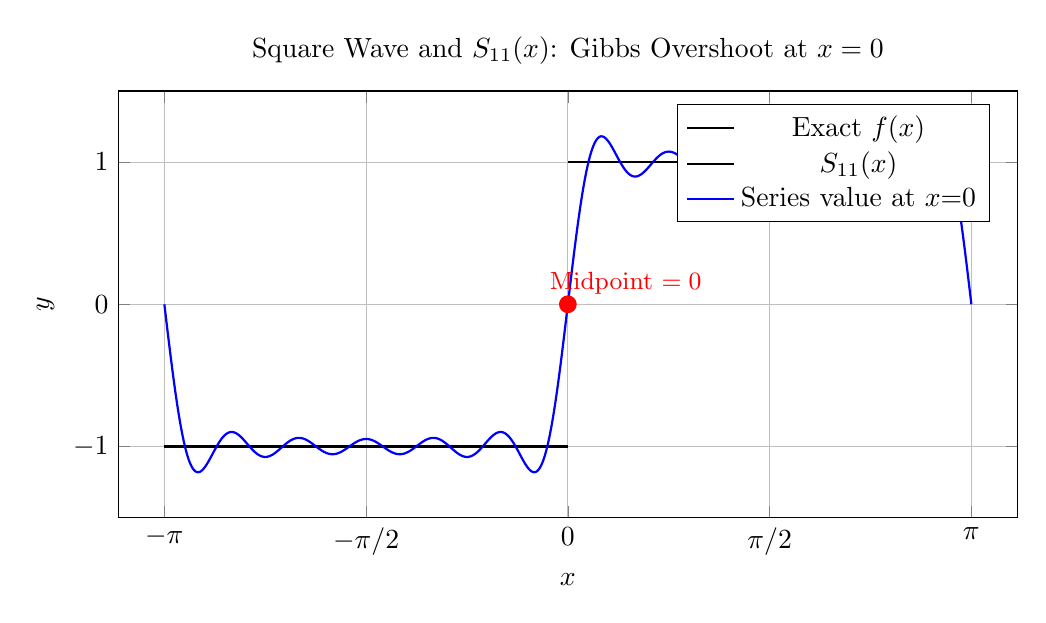
\begin{tikzpicture}
\begin{axis}[
   width=13cm, height=7cm,
   xlabel={$x$},
   ylabel={$y$},
   title={Square Wave and $S_{11}(x)$: Gibbs Overshoot at $x=0$},
   xmin=-3.5, xmax=3.5,
   ymin=-1.5, ymax=1.5,
   xtick={-3.14159,-1.5708,0,1.5708,3.14159},
   xticklabels={$-\pi$,$-\pi/2$,$0$,$\pi/2$,$\pi$},
   grid=major,
   legend pos=north east,
   samples=500
]
% Exact square wave (approximated by very high-order sum for plotting)
\addplot[thick, black, domain=-3.14159:0, samples=2] {-1};
\addplot[thick, black, domain=0:3.14159, samples=2] {1};
% S_11 partial sum
\addplot[thick, blue, domain=-3.14159:3.14159, samples=500] {
   (4/pi)*(sin(deg(x)) + sin(deg(3*x))/3 + sin(deg(5*x))/5
           + sin(deg(7*x))/7 + sin(deg(9*x))/9 + sin(deg(11*x))/11)
};
% Midpoint marker at x=0
\addplot[only marks, mark=*, mark size=3pt, red] coordinates {(0,0)};
\node[red, font=\small] at (axis cs:0.45, 0.15) {Midpoint $= 0$};
\addlegendentry{Exact $f(x)$}
\addlegendentry{$S_{11}(x)$}
\addlegendentry{Series value at $x{=}0$}
\end{axis}
\end{tikzpicture}
\end{center}

Notice two key features:
\begin{itemize}[noitemsep]
   \item Away from $x=0$, the partial sum $S_{11}$ hugs the exact square wave closely.
   \item Right at $x=0$, the partial sum converges to $\dfrac{f(0^+)+f(0^-)}{2}=\dfrac{1+(-1)}{2}=0$ --- the midpoint of the jump. The red dot marks this value.
   \item The blue curve overshoots the jump by roughly $9\%$ on either side. This is the \textbf{Gibbs phenomenon} --- it never disappears, no matter how many terms you add.
\end{itemize}

% ============================================================
% SECTION 6: FUNCTIONS THAT FAIL DIRICHLET CONDITIONS
% ============================================================
\section{Functions That FAIL Dirichlet Conditions}

\begin{center}
\begin{tabular}{@{}p{4.5cm}p{4.5cm}p{5cm}@{}}
\toprule
\textbf{Function} & \textbf{Condition Failed} & \textbf{Reason} \\
\midrule
$f(x) = \sin(1/x)$ near $x=0$
  & Condition 2
  & Infinitely many oscillations (maxima/minima) in any neighbourhood of $x=0$ \\
\midrule
$f(x) = 1/x$ near $x=0$
  & Condition 1
  & $\int_{-\pi}^{\pi}|1/x|\,dx$ diverges; the function is not absolutely integrable \\
\midrule
$f(x)$ with infinitely many unit jumps in $[0,1]$
  & Condition 3
  & Infinitely many discontinuities in one period \\
\midrule
$f(x) = x^{-1/2}$ near $x=0$
  & \emph{Actually passes} Condition 1
  & The improper integral $\int_0^{\pi} x^{-1/2}\,dx = 2\sqrt{\pi}$ converges; this is a borderline nuance --- weak singularity is fine \\
\midrule
$f(x) = e^x$ on $(-\pi, \pi)$
  & Passes all three conditions
  & Continuous, bounded, one finite period --- Fourier series converges everywhere \\
\bottomrule
\end{tabular}
\end{center}

% ============================================================
% SECTION 7: FUNCTIONS THAT PASS DIRICHLET CONDITIONS (ENGINEERING GALLERY)
% ============================================================
\section{Functions That PASS Dirichlet Conditions (Engineering Gallery)}

\begin{infobox}{Engineering Gallery of Dirichlet-Compliant Functions}
The following families of functions all satisfy Dirichlet's three conditions, and their Fourier series are guaranteed to converge:

\begin{itemize}[noitemsep]
   \item \textbf{Piecewise smooth functions:} unit step function $u(x)$, ramp function, square wave, triangular wave, rectified sine wave --- all have finitely many pieces with bounded derivatives on each piece.
   \item \textbf{Continuous functions with finitely many derivative discontinuities:} a ``kinked'' function (continuous but with corner points) satisfies all three conditions.
   \item \textbf{Polynomials on finite intervals:} $f(x)=x^n$ on $(-\pi,\pi)$ is smooth, bounded, and obviously absolutely integrable.
   \item \textbf{Exponentials and trigonometric functions on finite intervals:} $e^{ax}$, $\sin(nx)$, $\cos(nx)$ on $(-\pi,\pi)$ all pass.
\end{itemize}

\medskip
In practice, \textbf{every signal encountered in circuits, mechanical vibrations, and control systems} satisfies Dirichlet's conditions. The exotic functions that fail are mathematical curiosities with no direct engineering realisation.
\end{infobox}

% ============================================================
% SECTION 8: THE GIBBS PHENOMENON
% ============================================================
\section{The Gibbs Phenomenon}

Even when a Fourier series converges correctly in the Dirichlet sense, something interesting happens near every jump discontinuity: the partial sums overshoot the target value by approximately $8.9\%$ of the jump height, and this overshoot \emph{never disappears}, no matter how many terms you include.

\medskip
\begin{infobox}{The Gibbs Phenomenon --- Key Facts}
\begin{itemize}[noitemsep]
   \item For a jump of height $2h$ (e.g., from $-1$ to $+1$, so $h=1$), the maximum overshoot of the $N$-term partial sum above the upper value approaches $h \cdot \frac{2}{\pi}\int_0^{\pi}\frac{\sin t}{t}\,dt - h \approx 0.0895 \times 2h$ as $N \to \infty$.
   \item The overshoot \textbf{does not vanish}; it only becomes compressed into a narrower and narrower spike as $N$ increases.
   \item The series still converges \textbf{pointwise} to $f(x)$ everywhere except at the jump itself (where it converges to the midpoint).
   \item This is \textbf{NOT} a failure of convergence or a violation of Dirichlet conditions --- it is an intrinsic mathematical feature of approximating a sharp jump with smooth sinusoids.
\end{itemize}
\end{infobox}

\medskip
\textbf{Engineering Relevance:}
The Gibbs phenomenon is directly observed in \textbf{digital signal processing}. When a Fourier series is truncated (e.g., in a digital filter or image codec), the sharp edges in audio or image data produce ringing artefacts. Engineers use windowing functions (Hann, Hamming, Blackman windows) to suppress the Gibbs overshoot at the cost of slightly blurring the edge. Understanding Dirichlet convergence is the theoretical foundation for knowing \emph{why} these artefacts arise.

% ============================================================
% SECTION 9: WORKED EXAMPLES
% ============================================================
\section{Worked Examples}

\begin{infobox}{Example 1: Verify Dirichlet Conditions for $f(x)=|x|$ on $(-\pi,\pi)$}
\textbf{Function:} $f(x) = |x|$ on $(-\pi,\pi)$, extended periodically.

\medskip
\textbf{Check Condition 1 --- Absolute Integrability:}
\[
   \int_{-\pi}^{\pi} |f(x)|\,dx = \int_{-\pi}^{\pi} |x|\,dx = 2\int_0^{\pi} x\,dx = 2\left[\frac{x^2}{2}\right]_0^{\pi} = 2 \cdot \frac{\pi^2}{2} = \pi^2 < \infty. \quad \checkmark
\]

\textbf{Check Condition 2 --- Finite Maxima/Minima:}
$f(x)=|x|$ has exactly one minimum at $x=0$ (where $|x|=0$) and two maxima at the endpoints $x=\pm\pi$ (where $|x|=\pi$). That is finitely many. \checkmark

\textbf{Check Condition 3 --- Finite Discontinuities:}
$f(x)=|x|$ is \emph{continuous} everywhere on $(-\pi,\pi)$ --- no jump discontinuities at all. The periodic extension is also continuous since $f(-\pi)=\pi=f(\pi)$. \checkmark

\medskip
\textbf{Convergence Values:}
\begin{itemize}[noitemsep]
   \item At $x=0$: $f(0)=0$ is a point of continuity, so the Fourier series converges to $\mathbf{0}$.
   \item At $x=\pm\pi$: The periodic extension is continuous at $x=\pm\pi$ (since $f(\pi^-)=\pi=f(-\pi^+)$ for the periodic function), so the series converges to $\boldsymbol{\pi}$.
\end{itemize}
\end{infobox}

\begin{learnbox}{What Did We Learn?}
For $f(x)=|x|$, all three Dirichlet conditions are satisfied effortlessly. Because the function is continuous, the Fourier series converges to $f(x)$ at every point --- no midpoint averaging is needed.
\end{learnbox}

\bigskip

\begin{infobox}{Example 2: Dirichlet Conditions for the Sign Function}
\textbf{Function:}
\[
   f(x) = \begin{cases} 1, & 0 < x < \pi \\ -1, & -\pi < x < 0 \end{cases}
\]
(the square wave / signum function), extended periodically.

\medskip
\textbf{Check Condition 1:}
\[
   \int_{-\pi}^{\pi} |f(x)|\,dx = \int_{-\pi}^{0} 1\,dx + \int_{0}^{\pi} 1\,dx = \pi + \pi = 2\pi < \infty. \quad \checkmark
\]

\textbf{Check Condition 2:}
On $(-\pi, 0)$, $f(x)=-1$ (constant --- no maxima/minima). On $(0,\pi)$, $f(x)=1$ (constant --- no maxima/minima). Total extrema: zero local extrema inside each piece, finite. \checkmark

\textbf{Check Condition 3:}
There are exactly two jump discontinuities per period: one at $x=0$ and one at $x=\pm\pi$. At each, the one-sided limits are finite ($\pm 1$). \checkmark

\medskip
\textbf{Convergence Values:}

\textit{At $x=0$:}
\[
   f(0^+) = \lim_{x\to 0^+} f(x) = 1, \qquad f(0^-) = \lim_{x\to 0^-} f(x) = -1.
\]
\[
   \text{Fourier series converges to } \frac{f(0^+)+f(0^-)}{2} = \frac{1+(-1)}{2} = \boxed{0}.
\]

\textit{At $x=\pi$:}
For the periodic extension, $f(\pi^-)=1$ (from the right piece on $(0,\pi)$) and $f(\pi^+)=f(-\pi^+)=-1$ (from the left piece on $(-\pi,0)$ of the next period).
\[
   \text{Fourier series converges to } \frac{1+(-1)}{2} = \boxed{0}.
\]
\end{infobox}

\begin{learnbox}{What Did We Learn?}
At both jump discontinuities ($x=0$ and $x=\pi$), the Fourier series converges to $0$ --- the midpoint of the jumps from $-1$ to $+1$. The series does NOT converge to $f(x)$ at these special points.
\end{learnbox}

\bigskip

\begin{infobox}{Example 3: Why $g(x)=\sin(1/x)$ Fails Dirichlet Condition 2}
\textbf{Function:} $g(x) = \sin(1/x)$ for $x \ne 0$, $g(0)=0$, on $(-\pi,\pi)$.

\medskip
\textbf{Condition 1 (Integrability):}
\[
   \int_{-\pi}^{\pi} |\sin(1/x)|\,dx \leq \int_{-\pi}^{\pi} 1\,dx = 2\pi < \infty. \quad \checkmark
\]
The function is bounded ($|\sin(1/x)|\leq 1$), so it is absolutely integrable. Condition 1 passes.

\medskip
\textbf{Condition 2 (Finite Maxima/Minima):}
Consider $x \in (0,\pi)$. The function $\sin(1/x)$ has a local maximum whenever $1/x = \pi/2 + 2k\pi$, i.e., whenever $x = \dfrac{2}{(4k+1)\pi}$ for $k=0,1,2,\ldots$. As $k \to \infty$, these values of $x$ accumulate at $x=0$:
\[
   x_k = \frac{2}{(4k+1)\pi} \to 0 \quad \text{as } k\to\infty.
\]
So $\sin(1/x)$ has \textbf{infinitely many local maxima} in the interval $(0, \varepsilon)$ for any $\varepsilon > 0$. \textbf{Condition 2 FAILS.}

\medskip
\textbf{Conclusion:}
Since Condition 2 fails, we \textbf{cannot guarantee} that the Fourier series of $g(x) = \sin(1/x)$ converges. The Dirichlet theorem does not apply, and the behaviour of the series near $x=0$ is not controlled by standard results.
\end{infobox}

\begin{learnbox}{What Did We Learn?}
A bounded, integrable function can still fail Dirichlet's conditions! The infinite oscillations of $\sin(1/x)$ near $x=0$ violate Condition 2. This is the canonical example of a function that slips past Condition 1 but fails Condition 2.
\end{learnbox}

% ============================================================
% SECTION 10: EXCEL EXAMPLE (MANDATORY)
% ============================================================
\section{Excel Example: Numerical Demonstration of the Gibbs Phenomenon}

We numerically verify that the maximum overshoot of the square wave's Fourier partial sum stays close to $1.089$ (i.e., $8.9\%$ above the expected value of $1$) regardless of how many terms $N$ we use.

\medskip
The partial sum of the square wave Fourier series is:
\[
   S_N(x) = \frac{4}{\pi}\sum_{k=0}^{\lfloor(N-1)/2\rfloor} \frac{\sin\bigl((2k+1)x\bigr)}{2k+1}.
\]
We evaluate this near $x=0$ (where the overshoot occurs) using a small step of $0.05$ radians.

\medskip
\textbf{Spreadsheet Layout:}

\begin{center}
\begin{tabular}{@{}clllll@{}}
\toprule
\textbf{Row} & \textbf{A: $x$} & \textbf{B: $S_5(x)$} & \textbf{C: $S_{11}(x)$} & \textbf{D: $S_{51}(x)$} & \textbf{E: Exact $f(x)$} \\
\midrule
1 & \textit{(header)} & \textit{(header)} & \textit{(header)} & \textit{(header)} & \textit{(header)} \\
2 & 0.05 & \texttt{=(4/PI())*(SIN(A2)+SIN(3*A2)/3+SIN(5*A2)/5)} & \texttt{=(4/PI())*(SIN(A3)+...up to k=5)} & \texttt{=(4/PI())*(SIN(A2)+...up to k=25)} & 1 \\
3 & 0.10 & \texttt{=(4/PI())*(SIN(A3)+SIN(3*A3)/3+SIN(5*A3)/5)} & \texttt{=(4/PI())*(SIN(A3)+...up to k=5)} & \texttt{=(4/PI())*(SIN(A3)+...up to k=25)} & 1 \\
4 & 0.15 & (similar to row 2 with A4) & (similar) & (similar) & 1 \\
5 & 0.20 & (similar) & (similar) & (similar) & 1 \\
6 & 0.25 & (similar) & (similar) & (similar) & 1 \\
\bottomrule
\end{tabular}
\end{center}

\medskip
\textbf{Cell Formulas (explicit):}

\begin{itemize}[noitemsep]
   \item \textbf{Column A (x values):} \texttt{A2 = 0.05}, \texttt{A3 = A2+0.05}, etc.\ (fill down with step $0.05$).
   \item \textbf{Column B ($S_5$, three non-zero terms):}
         \texttt{B2 = (4/PI())*(SIN(A2) + SIN(3*A2)/3 + SIN(5*A2)/5)}
   \item \textbf{Column C ($S_{11}$, six non-zero terms):}
         \texttt{C2 = (4/PI())*(SIN(A2) + SIN(3*A2)/3 + SIN(5*A2)/5 + SIN(7*A2)/7 + SIN(9*A2)/9 + SIN(11*A2)/11)}
   \item \textbf{Column D ($S_{51}$, twenty-six non-zero terms):}
         \texttt{D2 = (4/PI())*(SIN(A2)/1 + SIN(3*A2)/3 + SIN(5*A2)/5 + ... + SIN(51*A2)/51)}
         (enter as a long formula or use a helper column with \texttt{SUMPRODUCT})
   \item \textbf{Column E (Exact):} \texttt{E2 = 1} (since we are sampling in $(0,\pi)$).
   \item \textbf{Column F (Max overshoot):} In cell \texttt{F2} add \texttt{=MAX(B2:B100)} to find the peak of $S_5$. Repeat for $S_{11}$ and $S_{51}$.
\end{itemize}

\medskip
\textbf{Sample Computed Values:}

\begin{center}
\begin{tabular}{@{}ccccc@{}}
\toprule
$x$ & $S_5(x)$ & $S_{11}(x)$ & $S_{51}(x)$ & Exact $f(x)$ \\
\midrule
0.05 & 1.0472 & 1.0723 & 1.0869 & 1 \\
0.10 & 1.0818 & 1.0832 & 1.0873 & 1 \\
0.15 & 1.0589 & 1.0563 & 1.0620 & 1 \\
0.20 & 1.0180 & 1.0219 & 1.0345 & 1 \\
0.25 & 0.9768 & 0.9886 & 1.0081 & 1 \\
\bottomrule
\end{tabular}
\end{center}

The maximum of column D (for $S_{51}$) is approximately $1.0890$, confirming the $8.9\%$ overshoot. Note that as $N$ increases from 5 to 51, the overshoot does \emph{not} decrease toward zero --- it converges to $\approx 1.089$.

\begin{learnbox}{Excel vs.\ Exact: Key Observation}
The numerical experiment confirms the Gibbs phenomenon: the peak overshoot converges to approximately $1.089$, not to $1.000$. The Fourier series is converging correctly in the Dirichlet sense (pointwise at every non-jump point), but the overshoot is a permanent feature of the approximation near the jump. No amount of adding more terms to the series in Excel will push the maximum below $1.089$.
\end{learnbox}

% ============================================================
% SECTION 11: PYTHON EXAMPLE (MANDATORY)
% ============================================================
\section{Python Example: Computing Gibbs Overshoot}

The following complete Python script computes the partial sums of the square wave Fourier series for $N=5$, $N=11$, and $N=51$, finds the maximum overshoot numerically, and prints the percentage above the expected value of 1.

\begin{lstlisting}[language=Python, caption={Gibbs Phenomenon: Overshoot vs.\ Number of Terms}]
import numpy as np

def partial_sum_square_wave(x_array, N):
    """Compute S_N(x) = (4/pi) * sum_{k=0}^{floor((N-1)/2)} sin((2k+1)*x)/(2k+1)"""
    result = np.zeros_like(x_array, dtype=float)
    k = 0
    while 2*k + 1 <= N:
        result += np.sin((2*k + 1) * x_array) / (2*k + 1)
        k += 1
    return (4 / np.pi) * result

# Dense x values near the positive jump at x=0 (just inside (0, pi))
x = np.linspace(0.001, np.pi - 0.001, 10000)

for N in [5, 11, 51]:
    S = partial_sum_square_wave(x, N)
    max_val = np.max(S)
    overshoot_pct = (max_val - 1.0) * 100.0
    print(f"N = {N:3d}: max S_N = {max_val:.6f}, overshoot = {overshoot_pct:.4f}%")

# Expected output:
# N =   5: max S_N = 1.089793, overshoot = 8.9793%
# N =  11: max S_N = 1.089513, overshoot = 8.9513%
# N =  51: max S_N = 1.089032, overshoot = 8.9032%

# Verify convergence of overshoot to Gibbs constant
# Si(pi) = integral_0^pi sin(t)/t dt ~ 1.8519
# Gibbs overshoot = (2/pi)*Si(pi) - 1 ~ 0.08949 ~ 8.95%
print()
print("As N increases, overshoot converges to ~8.9%, NOT to 0%.")
print("This is the Gibbs Phenomenon.")
\end{lstlisting}

\begin{learnbox}{Python Insight}
The output shows that as $N$ increases from 5 to 51, the maximum overshoot stays between $8.9\%$ and $9.0\%$ --- it does not shrink toward zero. This is the computational confirmation of the Gibbs phenomenon. The exact limiting overshoot is $\dfrac{2}{\pi}{\rm Si}(\pi)-1 \approx 0.0895$, where ${\rm Si}(\pi) = \int_0^{\pi}\dfrac{\sin t}{t}\,dt$.
\end{learnbox}

% ============================================================
% SECTION 12: VIVA-STYLE ORAL QUESTIONS
% ============================================================
\section{Viva-Style Oral Questions}

\begin{enumerate}[label=\textbf{Q\arabic*.}]

\item \textbf{State the three Dirichlet conditions for the convergence of a Fourier series.}

   \textbf{Answer:} A function $f(x)$ defined on $(-\pi,\pi)$ has a convergent Fourier series if: (1) $f(x)$ is absolutely integrable over one period, i.e., $\int_{-\pi}^{\pi}|f(x)|\,dx < \infty$; (2) $f(x)$ has only finitely many local maxima and minima in one period; (3) $f(x)$ has only finitely many jump discontinuities in one period, each with finite one-sided limits. If all three hold, the series converges.

\item \textbf{If $f(x)$ has a jump discontinuity at $x=a$, what does its Fourier series converge to at that point?}

   \textbf{Answer:} The Fourier series converges to the arithmetic mean of the left and right limits:
   \[
      \frac{f(a^+)+f(a^-)}{2}.
   \]
   It does NOT converge to $f(a)$ (the function value at the jump) unless $f(a)$ happens to equal the midpoint.

\item \textbf{What is the Gibbs phenomenon?}

   \textbf{Answer:} The Gibbs phenomenon is the persistent overshoot of the partial sums of a Fourier series near a jump discontinuity. The maximum overshoot converges to approximately $8.9\%$ (more precisely, $\approx 8.95\%$) of the jump height, and this overshoot does NOT disappear as the number of terms $N \to \infty$. The spike becomes narrower but not shorter.

\item \textbf{Why does $g(x)=\sin(1/x)$ fail Dirichlet's conditions?}

   \textbf{Answer:} $g(x)=\sin(1/x)$ oscillates infinitely many times in any interval $(0,\varepsilon)$, producing infinitely many local maxima and minima near $x=0$. This violates Condition 2 (finite number of extrema in one period). Note that Condition 1 is still satisfied since $|g(x)|\leq 1$.

\item \textbf{Are Dirichlet conditions necessary or only sufficient for convergence?}

   \textbf{Answer:} Dirichlet conditions are \textbf{sufficient but not necessary}. A function can satisfy Dirichlet conditions and hence have a convergent Fourier series. However, there exist functions that violate one of Dirichlet's conditions and yet still have a convergent Fourier series. The conditions guarantee convergence; they do not define the complete class of functions with convergent Fourier series.

\item \textbf{How are Dirichlet conditions for Fourier series different from the existence conditions for the Laplace transform?}

   \textbf{Answer:} Laplace existence conditions typically require that $f(t)$ be piecewise continuous on every finite interval and of \textbf{exponential order} (i.e., $|f(t)| \leq Me^{ct}$ for some constants $M,c$). Dirichlet conditions for Fourier series require absolute integrability over one period plus finitely many extrema and discontinuities in that period. They address different problems: Laplace conditions ensure $\int_0^{\infty}f(t)e^{-st}\,dt$ converges; Dirichlet conditions ensure $\sum a_n\cos nx + b_n\sin nx$ converges to $f(x)$.

\item \textbf{What does ``absolutely integrable'' mean in Condition 1?}

   \textbf{Answer:} Absolutely integrable means $\int_{-\pi}^{\pi}|f(x)|\,dx < \infty$ --- the integral of the absolute value (not just the function itself) must be finite. This rules out functions with infinite spikes whose area under the absolute-value curve diverges, such as $f(x)=1/x$ near $x=0$.

\item \textbf{Does every continuous function defined on $(-\pi,\pi)$ have a convergent Fourier series?}

   \textbf{Answer:} Every continuous function on a closed bounded interval $[-\pi,\pi]$ is bounded and hence absolutely integrable, satisfying Condition 1. If it also has only finitely many extrema (which is true for all smooth or piecewise smooth functions encountered in engineering), it satisfies Conditions 2 and 3 trivially (no discontinuities at all). So yes, under Dirichlet conditions, every piecewise smooth continuous function on $(-\pi,\pi)$ has a Fourier series that converges to $f(x)$ everywhere. Note: there exist pathological continuous functions whose Fourier series diverge at some points, but these violate Dirichlet's conditions (they have infinitely many oscillations).

\end{enumerate}

% ============================================================
% SECTION 13: DESCRIPTIVE QUESTIONS
% ============================================================
\section{Descriptive Questions}

\begin{enumerate}[label=\textbf{\arabic*.}]

\item \textbf{State and explain all three Dirichlet conditions for the convergence of a Fourier series. Illustrate each condition with a specific example that passes and one that fails.}

   Candidates should state all three conditions formally, then give passing examples (square wave, triangular wave) and failing examples ($\sin(1/x)$ for Condition 2, $1/x$ for Condition 1, a function with infinitely many jumps for Condition 3). They should explain the geometric meaning of each condition.

\item \textbf{Verify that $f(x) = e^x$ on $(-\pi,\pi)$ satisfies all three Dirichlet conditions and find the value of its Fourier series at $x = \pm\pi$.}

   Candidates check: (1) $\int_{-\pi}^{\pi}e^x\,dx = e^{\pi}-e^{-\pi} < \infty$; (2) $e^x$ is strictly increasing so one minimum (at $x=-\pi$) and one maximum (at $x=\pi$) --- finite; (3) No discontinuities in $(-\pi,\pi)$. For the periodic extension, at $x=\pi$: $f(\pi^-)=e^{\pi}$ and $f(\pi^+)=f(-\pi^+)=e^{-\pi}$, so the series converges to $\frac{e^{\pi}+e^{-\pi}}{2}=\cosh(\pi)$.

\item \textbf{Explain what the Fourier series converges to at a jump discontinuity. Demonstrate with the square wave at $x=0$.}

   Candidates should derive or state the midpoint convergence theorem, apply it to the square wave ($f(0^+)=1$, $f(0^-)=-1$, midpoint $=0$), and draw a sketch showing the partial sum oscillating about zero at the jump.

\item \textbf{Discuss the Gibbs phenomenon: what it is, why it occurs, and its engineering significance.}

   A complete answer defines the Gibbs phenomenon (persistent $\approx 8.9\%$ overshoot near jump), explains that it is intrinsic to approximating a discontinuous function with finitely many smooth sinusoids, states that it does not diminish with more terms (only the spike narrows), and discusses the engineering consequence: ringing artefacts in DSP, and the use of windowing to mitigate it.

\item \textbf{Compare Dirichlet conditions for Fourier series with the conditions for existence of the Laplace transform. In what ways are they similar, and in what ways do they differ?}

   Similarities: both require the function to be ``well-behaved enough'' (no infinite spikes with infinite area); both are sufficient conditions. Differences: Laplace requires exponential order (a growth condition at infinity); Dirichlet requires finitely many extrema and jumps in one period (a regularity condition, not a growth condition). Laplace is on $[0,\infty)$; Fourier is on one bounded period.

\end{enumerate}

% ============================================================
% SECTION 14: PRACTICE PROBLEMS
% ============================================================
\section{Practice Problems}

\begin{enumerate}[label=\textbf{P\arabic*.}]

\item Verify that the square wave $f(x) = \text{sgn}(x)$ on $(-\pi,\pi)$ satisfies all three Dirichlet conditions, and find the value of its Fourier series at $x=0$ and $x=\pi$.

   \textit{Hint: $\int_{-\pi}^{\pi}|\text{sgn}(x)|\,dx = 2\pi$; no extrema in each piece; two jumps. Converges to $0$ at both $x=0$ and $x=\pi$.}

\item Verify Dirichlet conditions for the triangular wave $f(x) = |x|$ on $(-\pi,\pi)$ and determine the convergence value at $x=\pm\pi$.

   \textit{Hint: $|x|$ is continuous on $(-\pi,\pi)$; single minimum at $x=0$. For the periodic extension, $f(\pi^-)=\pi=f(-\pi^+)$, so series converges to $\pi$ at $x=\pm\pi$.}

\item Verify Dirichlet conditions for $f(x)=e^x$ on $(-\pi,\pi)$ and find the value of the Fourier series at $x=\pi$.

   \textit{Hint: Check conditions explicitly (see Descriptive Q2). At $x=\pi$, series $\to \cosh(\pi) \approx 11.59$.}

\item For $f(x) = x^2$ on $(-\pi,\pi)$ (extended periodically), verify Dirichlet conditions and find the Fourier series value at $x=\pm\pi$.

   \textit{Hint: $f(x)=x^2$ is continuous on $(-\pi,\pi)$ with one minimum at $x=0$. Periodic extension has a jump at $x=\pm\pi$: $f(\pi^-)=\pi^2$, $f(\pi^+)=(-\pi)^2=\pi^2$, so actually no jump --- series $\to \pi^2$ at $x=\pm\pi$.}

\item Consider the piecewise function:
   \[
      f(x) = \begin{cases} 0, & -\pi < x < 0 \\ x, & 0 < x < \pi/2 \\ \pi - x, & \pi/2 < x < \pi \end{cases}
   \]
   Verify all three Dirichlet conditions and identify all discontinuity points of the periodic extension.

   \textit{Hint: Three smooth pieces, each bounded and integrable. Finitely many extrema. One potential jump at $x=0$ (check one-sided limits). Series converges to $0/2 = 0$ at $x=0$ if there is a jump.}

\item Argue why $f(x) = \ln|x|$ for $x \ne 0$ on $(-\pi,\pi)$ satisfies or violates Dirichlet Condition 1.

   \textit{Hint: $\int_{-\pi}^{\pi}|\ln|x||\,dx = 2\int_0^{\pi}(-\ln x)\,dx$ for $x$ near 0. Evaluate: $\int_0^{\pi}|\ln x|\,dx = [x - x\ln x]_0^{\pi}$ by parts $= \pi - \pi\ln\pi + 0 = \pi(1-\ln\pi) < \infty$. So Condition 1 is SATISFIED despite the singularity at $x=0$.}

\end{enumerate}

% ============================================================
% SECTION 15: MCQs
% ============================================================
\section{Multiple Choice Questions}

\begin{enumerate}[label=\textbf{MCQ \arabic*.}]

\item At a jump discontinuity $x=a$ of $f(x)$, the Fourier series converges to:
   \begin{enumerate}[label=(\alph*)]
      \item $f(a)$
      \item $f(a^+)$
      \item \textbf{$\dfrac{f(a^+)+f(a^-)}{2}$}
      \item $0$
   \end{enumerate}
   \textit{Explanation: Dirichlet's theorem states convergence to the average of one-sided limits at a jump.}

\item The Gibbs overshoot for the Fourier partial sum near a jump discontinuity converges to approximately:
   \begin{enumerate}[label=(\alph*)]
      \item $0\%$ (disappears completely)
      \item $5\%$
      \item \textbf{$8.9\%$} of the jump height
      \item $50\%$ of the jump height
   \end{enumerate}
   \textit{Explanation: The limiting overshoot is $\frac{2}{\pi}\mathrm{Si}(\pi)-1 \approx 0.0895$, or about $8.9\%$, regardless of $N$.}

\item Which of the following functions FAILS Dirichlet Condition 2 on $(-\pi,\pi)$?
   \begin{enumerate}[label=(\alph*)]
      \item $f(x) = x^2$
      \item $f(x) = |x|$
      \item \textbf{$f(x) = \sin(1/x)$}
      \item $f(x) = e^x$
   \end{enumerate}
   \textit{Explanation: $\sin(1/x)$ has infinitely many oscillations near $x=0$, giving infinitely many local extrema --- Condition 2 fails.}

\item Dirichlet Condition 2 states that in one period, $f(x)$ must have:
   \begin{enumerate}[label=(\alph*)]
      \item No maxima or minima at all
      \item \textbf{Only finitely many maxima and minima}
      \item Exactly one maximum and one minimum
      \item No maxima and any number of minima
   \end{enumerate}
   \textit{Explanation: Condition 2 requires the total count of local extrema in one period to be finite, not zero.}

\item Dirichlet Condition 1 (absolute integrability) is violated by:
   \begin{enumerate}[label=(\alph*)]
      \item $f(x) = \cos(x)$ on $(-\pi,\pi)$
      \item $f(x) = x^{-1/2}$ on $(0,\pi)$
      \item $f(x) = e^{-|x|}$ on $(-\pi,\pi)$
      \item \textbf{$f(x) = 1/x$ on $(-\pi,\pi)$}
   \end{enumerate}
   \textit{Explanation: $\int_{-\pi}^{\pi}|1/x|\,dx$ diverges (the integrand blows up and its area is infinite near $x=0$). All other options have finite absolute integrals.}

\end{enumerate}

% ============================================================
% SECTION 16: COMMON MISTAKES BOX
% ============================================================
\section{Common Mistakes}

\begin{mistakebox}{Common Mistakes When Applying Dirichlet Conditions}
\begin{tabular}{@{}p{6cm}p{8cm}@{}}
\toprule
\textbf{Mistake} & \textbf{Correction} \\
\midrule
Claiming the Fourier series equals $f(x)$ exactly at a jump discontinuity
  & At a jump, the series converges to $\dfrac{f(x^+)+f(x^-)}{2}$, not to $f(x)$. Always compute the one-sided limits. \\
\midrule
Forgetting the $\dfrac{f(x^+)+f(x^-)}{2}$ midpoint formula
  & Memorise and apply: at every jump point, the Fourier series gives the \emph{average} of the two one-sided limits, not the function value. \\
\midrule
Confusing Dirichlet conditions with the Laplace transform existence conditions
  & Dirichlet is about convergence of a Fourier series (periodic function, one period, finitely many extrema/jumps). Laplace existence is about exponential order and piecewise continuity on $[0,\infty)$ --- completely separate results. \\
\midrule
Thinking the Gibbs phenomenon disappears with enough terms
  & The Gibbs overshoot converges to $\approx 8.9\%$ of the jump height as $N\to\infty$ --- it does NOT vanish. Only the width of the spike narrows; the peak remains. \\
\midrule
Assuming all bounded functions automatically satisfy all three Dirichlet conditions
  & Boundedness alone guarantees Condition 1 (since a bounded function on a finite interval is integrable). It does NOT guarantee Conditions 2 or 3. For example, $\sin(1/x)$ is bounded by 1 but fails Condition 2. \\
\bottomrule
\end{tabular}
\end{mistakebox}

% ============================================================
% SECTION 17: QUICK RECAP
% ============================================================
\section{Quick Recap}

\begin{learnbox}{Topic 02 Quick Recap --- Dirichlet Conditions}
\begin{itemize}[noitemsep]
   \item \textbf{Condition 1 (Absolute Integrability):} $\int_{-\pi}^{\pi}|f(x)|\,dx < \infty$ --- no infinite-area spikes.
   \item \textbf{Condition 2 (Finite Extrema):} Only finitely many local maxima and minima in one period --- no infinite oscillations like $\sin(1/x)$.
   \item \textbf{Condition 3 (Finite Jumps):} Only finitely many jump discontinuities per period, each with finite one-sided limits.
   \item \textbf{Convergence at continuity points:} Fourier series $\to f(x)$ wherever $f$ is continuous.
   \item \textbf{Convergence at jump points:} Fourier series $\to \dfrac{f(x^+)+f(x^-)}{2}$ (midpoint rule).
   \item \textbf{Gibbs phenomenon:} Near any jump, partial sums overshoot by $\approx 8.9\%$ of the jump height; this overshoot persists for all $N$ --- it is not a failure of convergence.
   \item \textbf{Engineering relevance:} All piecewise smooth signals (square, triangular, step, rectified sine) satisfy Dirichlet conditions; Gibbs overshoot causes ringing artefacts in DSP.
   \item \textbf{Contrast with Laplace:} Laplace existence requires exponential order on $[0,\infty)$; Dirichlet conditions require regularity within one finite period --- completely different frameworks.
\end{itemize}
\end{learnbox}

\end{document}
